\chapter{Hibrid szimulációs módszer}\label{chap:hibrid}

{\ }


A hibrid szimulációs módszer a numerikus számítások és a kísérleti eljárások előnyeinek ötvözésén alapul.  A módszer alapötlete még a '70-es évekből származik, azonban az irányítástechnikai fejlettség és a számítógépek  kapacitása csak  nagyjából a 2000-es évektől tette lehetővé elterjedését. A fejlődésben nagy előrelépést jelentett a CR algoritmus megjelenése és sikeres alkalmazása a hibrid vizsgálatokra.  Napjainkban az igény is megnőtt rá, mivel a földrengésre vonatkozó tervezési alapelvek sokkal szigorúbb követelményeket támasztanak, és a védekezési és kockázatcsökkentési módszerek között előtérbe kerültek  az olyan összetett viselkedésű szerkezeti  megoldások, mint az aktív és passzív kontroll rendszerek. Ezek  vizsgálatára a legjobban  a hibrid módszer alkalmas, mivel nagy fölénnyel bír más módszerekhez képest a bonyolult, nemlineáris viselkedésű elemeket is tartalmazó szerkezetek vizsgálatában, a numerikus és a kísérleti vizsgálati eljárások ilyen esetekben nem alkalmazhatók hatékonyan.

A numerikus számítások egyik nagy hátránya, hogy időigényesek, ha nemlineáris módszert kell alkalmazni. Mint azt a \ref{sec:nl idolepmsz} pontban is bemutattuk, a nemlineáris időlépéses módszerek sokkal bonyolultabbak a lineáris algoritmusoknál. Ilyenkor a merevségi mátrix helyett az elmozdulásfüggő visszatérítő erővel számolunk, amit minden egyes időlépésben felül kell írnunk, így jelentősen megnő a számítás ideje.
 
A numerikus számítások ellen szól az is, hogy a szerkezetekben sokszor alkalmaznak olyan másodlagos teherviselő elemeket (pl. merevítők, vékonyfalú  szelemenek, kihajlásbiztos rudak), amelyeknek a gazdaságosság végett kihasználják a képlékeny tartalékait. Jelenleg a képlékeny vizsgálatokra még nincs kellően pontos dinamikus modellünk, ezért a kísérleti analízis több és biztosabb információval szolgálhat.

A nemlineáris vizsgálatok előtérbe kerülésének még egy oka az építőiparban felhasznált anyagok fejlődése. Egyre nagyobb szilárdságú anyagokat alkalmazunk, ezáltal karcsúbbak a  szerkezetek, és a másodrendű hatások szerepe megnő. Mivel a másodrendű hatásokra  sincsenek kellőképp jól alkalmazható modellünk, az ilyen szerkezetek viselkedését is kísérleti módszerekkel célszerű vizsgálni.

Azonban nem hagyhatjuk figyelmen kívül, hogy a kísérleti eljárásoknak is megvannak a hátrányai. A legfőbb probléma, hogy dinamikus terhelés esetén  általában 1:1 arányú modellt célszerű  vizsgálni, ezért a teljes szerkezet megépítése meglehetősen költséges  és helyigényes. A megfelelő laboratóriumi körülmények megteremtése is bonyolult  feladat, mivel nagy és drága  mozgató szerkezetet kell biztosítani. Esetenként ennek vonzata lehet a laboratórium tartószerkezetének megerősítése is, ráadásul a vizsgáló berendezések kezelése szakképzett munkaerőt igényel. 

További hátrányt jelent, hogy fenntartási szempontból  olyan szerkezetet célszerű tervezni, amiben a képlékeny alakváltozások lokalizáltak és könnyen ellenőrizhetők. Ezért a szerkezetek többségében csak néhány elem rendelkezik képlékeny, nemlineáris tulajdonságokkal, a többi elem általában lineárisan viselkedik. Ezek modellezése és numerikus analízise egyszerűbb, a lineáris megoldókkal nem jelent kihívást. A teljes szerkezeti modell vizsgálata ezért feleslegessé válik, hiszen csak a képlékeny tartalékkal bíró elemek viselkedését lenne szükséges megfigyelni.  

Ezek az érvek együttesen egy olyan kísérleti  módszer igényét mutatják, ahol a szerkezet elemzését felosztják párhuzamosan futó laboratóriumi vizsgálatra és  numerikus analízisre.  Erre fejlesztették a hibrid szimulációs módszert, melynek lényege, hogy  a lineáris viselkedésű szerkezeti részeket numerikusan modellezzük, a nemlineáris, nem ismert viselkedésű elemeket pedig laborban kísérleti úton vizsgáljuk. A szerkezetet az alszerkezetek módszerével osztjuk fel a numerikus és a kísérleti alszerkezetre, és a két rész között folyamatos adatátvitelt biztosítunk. 

A hibrid szimulációnak több alkalmazási módja is elterjedt. Ezek osztályozhatók például  földrajzi helyzetük és  vizsgálati sebességük szerint is. Földrajzi elhelyezkedésük tekintetében beszélhetünk helyi szimulációról, amikor a numerikus és fizikai szerkezeti részek mind egy laboratóriumban helyezkednek el, illetve földrajzilag megosztott hibrid szimulációról, amikor a numerikus és kísérleti analízis egyszerre több részletben több  laboratóriumban zajlik.

Egy másik osztályozási lehetőség a szimuláció sebessége alapján történő besorolás. A vizsgálat időléptéke  a valós időléptéknél kétszer lassabb, és sokszor gyorsabb intervallum között változhat. Ezek alapján megkülönböztethetünk lassú, gyors és valós idejű vizsgálatokat. A lassú vizsgálatok előnye, hogy könnyebben megfigyelhetők a vizsgált  folyamatok, viszont a sebesség csökkentéséből adódóan a vizsgálat pontossága is csökken. A valós idejű szimulációk ezzel szemben pontos vizsgálatot tesznek lehetővé, de a rendszert leíró mozgásegyenletek ekkor bonyolultabbá válnak, megoldásuk nehezebb, és a szimuláció végrehajtása számos  irányítástechnikai problémát is felvet. 

A következőkben a hibrid szimuláció legfontosabb kérdéseit járom körül Schellenberg, Mahin és Fenves  munkája alapján \cite{hibrid}. Először a főbb, mai gyakorlatban alkalmazott kísérleti módszereket ismertetem, utoljára hagyva a hibrid szimulációs eljárást.   Ezután a hibrid szimuláció előnyeit és a szimulációval kapcsolatos legfontosabb kihívásokat foglalom össze, majd  a szimuláció kulcselemeit és folyamatát vázolom. Végül a különböző osztályozási lehetőségeit ismertetem a kísérlet földrajzi megosztottsága és a szimuláció gyorsasága szerint. 
 
\section{A legtöbbet alkalmazott kísérleti eljárások}

{\ }
 
Jelenleg számos bevált laboratóriumi kísérleti módszer létezik a szerkezeti rendszerek vagy azok összetevőinek szeizmikus  viselkedésének vizsgálatára. A legelterjedtebb módszer a kvázi-statikus vizsgálati módszer, ahol a vizsgált szerkezetet előre meghatározott teher- vagy elmozdulástörténetnek vetik alá valamilyen aktuátor segítségével. Azáltal, hogy ugyanazt a terhet vagy elmozdulást több mintadarabon működtetjük, az anyagi tulajdonságok, részletek, peremfeltételek, terhelési arányok és más tényezők szisztematikus változásai könnyen beazonosíthatók. Ez a vizsgálati módszer gazdaságos és viszonylag egyszerű, azonban  a   próbatestekre vonatkozó általános követelmények nem kapcsolódnak közvetlenül a megfigyelt károkhoz, ami kérdéseket vet fel terv-specifikus helyzetekben, továbbá az alkalmazott terhelésminták általában nem alkalmasak a szeizmikus hatás okozta terhelés szimulációjára. Az \ref{fig:quasi} ábrán egy falazaton végzett kvázi-statikus vizsgálat felállása látható.  A kísérlet előtt a kutatócsoport tagjai, A. Salmanpour, N.  Mojsilovic és J. Schwartz láthatók. A  kísérletet a Zürichi Szövetségi Műszaki Intézetben (ETH) végezték. A képen jól  megfigyelhetők a vizsgálóberendezés  méretei. 

\begin{figure}[h!bt]
\centering
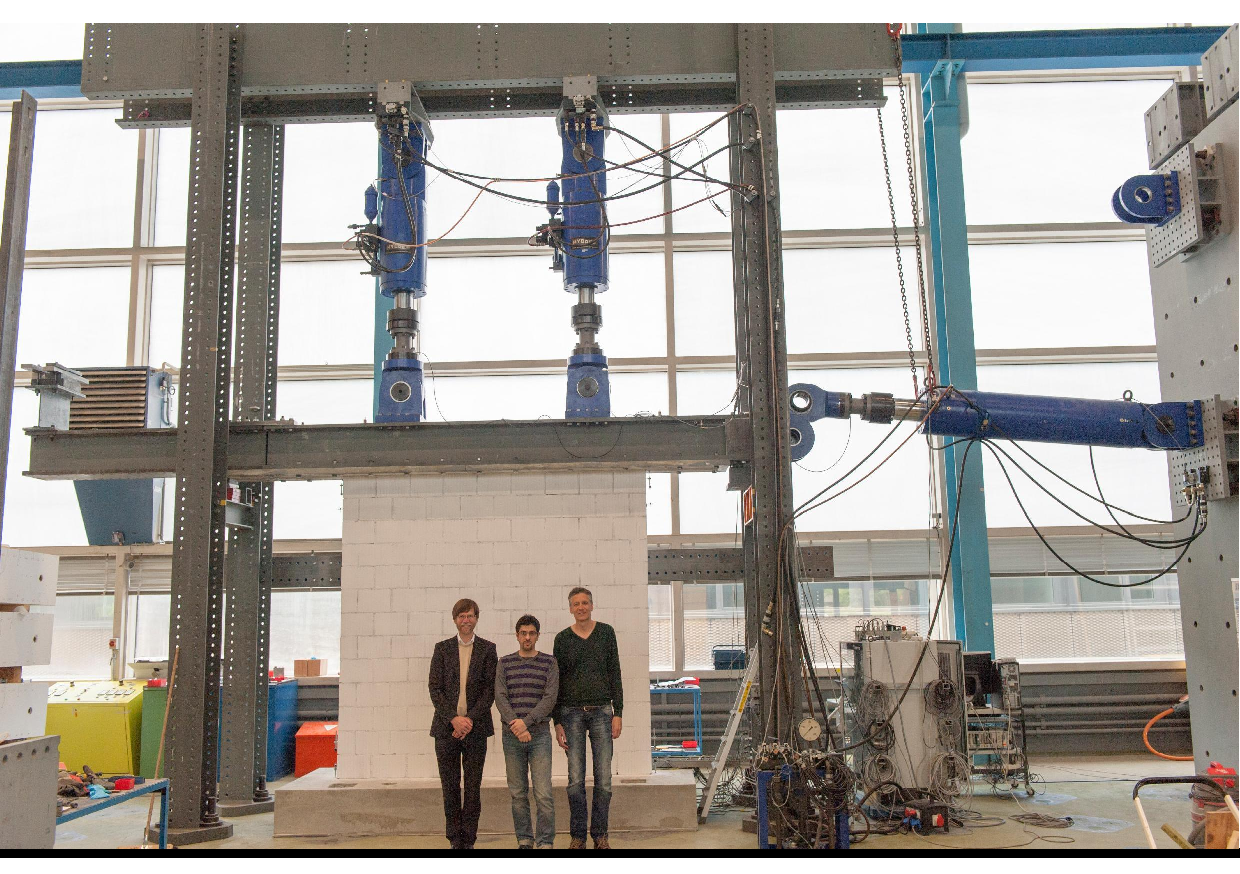
\includegraphics[width=\textwidth]{quasi_stati.pdf}
\caption{Falazat kvázi-statikus vizsgálata \cite{quasi}.}
\label{fig:quasi}
\end{figure}


A rázópad-vizsgálat a második legelterjedtebb formája a laborkísérleteknek. A valós földrengések alatti állapotokhoz hasonlót lehet szimulálni a vizsgálattal. A rázópad-kísérletek fontos adatokat szolgálnak a földrengésekre adott dinamikus válaszokról, figyelembe véve a vizsgált szerkezet inerciáit és energia-disszipációit, valamint a geometriai nemlinearitások, a korlátozott alakváltozások  és a szerkezeti elemek meghibásodásának következményeit. A módszer hátránya, hogy a teljes szerkezeti rendszert gondosan fel kell építeni. Másrészt viszont a  valós idejű dinamikus elem vizsgálat számos lehetőséget tartogat, azonban irányítása komoly kihívást jelent, mert a rázópad mozgatását ekkor aktuátorok végzik.  A rázópadok korlátozott méretei és kapacitása miatt a próbatestek mérete, súlya és teherbírása is jelentősen korlátozott, ennek eredményeként gyakran csökkentett méretű vagy nagyon leegyszerűsített próbadarabok válnak szükségessé, és ezért sokszor megkérdőjelezhetővé válnak a vizsgálati eredmények.
Az \ref{fig:shaking} ábrán egy hatszabadságfokú rázópad látható. A szerkezet a George Washington Egyetem (GWU) laboratóriumában található.

\begin{figure}[h!bt]
\centering
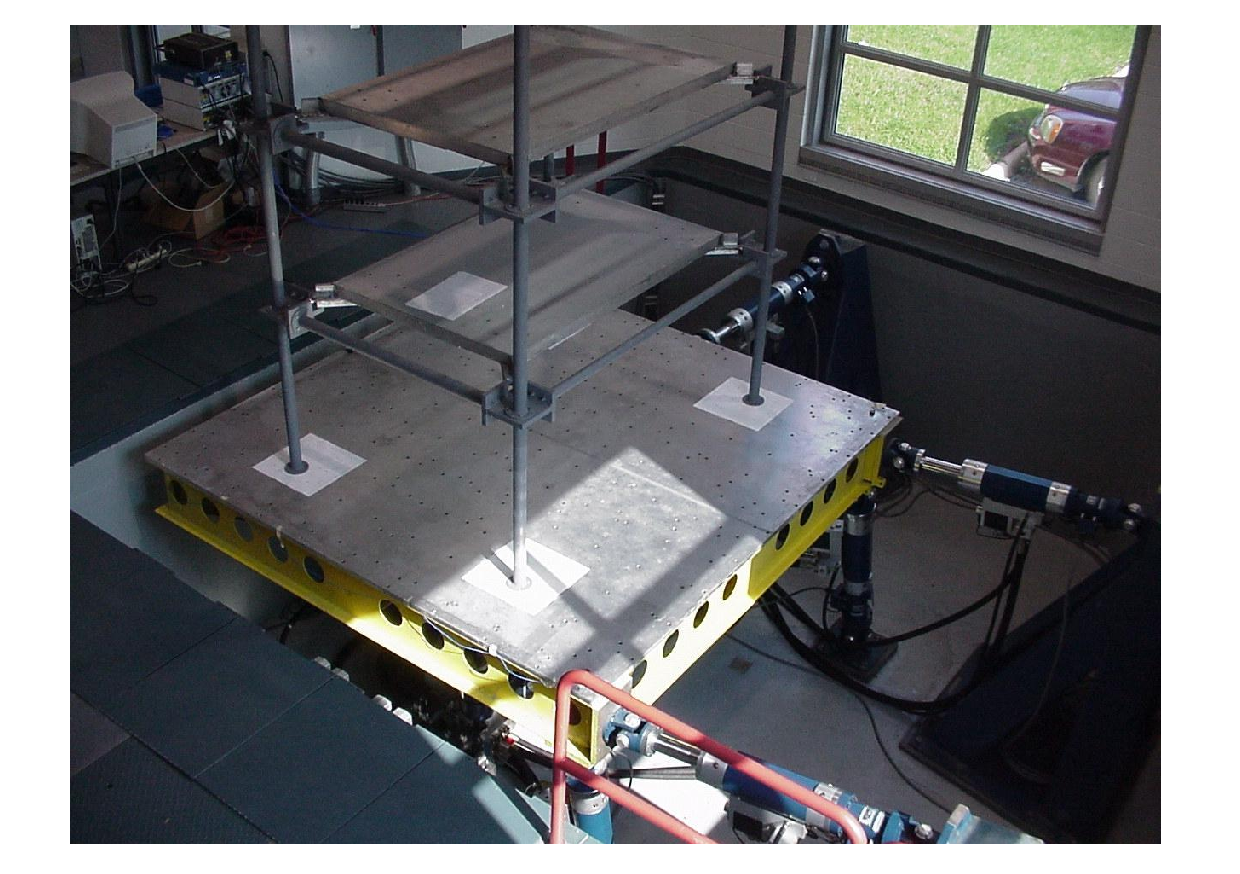
\includegraphics[width=\textwidth]{Shake_Table.pdf}
\caption{Hatszabadságfokú rázópad \cite{shaking}.}
\label{fig:shaking}
\end{figure}

A harmadik módszer a hibrid szimuláció, más néven pszeudo-dinamikus vagy csatolt számítógép-irányított vizsgálati módszer. Ebben a  kísérleti eljárásban a szimuláció egy olyan modellen van végrehajtva, ami figyelembe veszi a szerkezet numerikus és fizikai komponenseit is, és az erre felírt mozgásegyenletek  időlépéses numerikus megoldásán alapul. A hagyományos számítógépes modellezéssel és szimulációval ellentétben, ahol az egész szerkezet analitikusan van elemezve, a hibrid szimulációs módszerben  a szerkezeti rendszer erőjellegű mennyiségei dinamikus terhelés esetén (mint a merevség, energia-disszipáció vagy tömeg tulajdonságok)  a teljes szerkezetnek vagy egyes részeinek laboratóriumi vizsgálatával válnak ismertté. Ha a hibrid szimuláció egy szokványos kvázi-statikus elmozdulásalapú vizsgálatként van végrehajtva, a próbatest tömeg- és viszkózus csillapításjellemzői numerikusan modellezhetők, és a szerkezet meghatározott dinamikus gerjesztésének hatására keletkező elmozdulásnövekmények minden lépésnél a fizikai és numerikus modellek alapján számíthatók. A szimuláció során a teljes hibrid modell fizikai részei egy vagy több laboratóriumban vizsgálhatók számítógép-irányított aktuátor segítségével, és egyidejűleg a numerikus részek egy vagy több számítógépen analizálhatók. Mivel a szimuláció dinamikus aspektusai numerikusan vannak kezelve, az ilyen vizsgálatok kvázi-statikusan végezhetők hagyományos számítógép-irányított aktuátort használva. A hibrid szimulációt ezért úgy is lehet tekinteni, mint egy speciális aktuátor alapú vizsgálatot, ahol a terheléstörténet egy kísérlet során van meghatározva, melyben a szerkezet adott földmozgásnak van alávetve. Másrészről a hibrid szimuláció felfogható hagyományos végeselemes vizsgálatnak is, ahol a numerikus modellbe be van ágyazva a szerkezet egyes részeinek fizikai modellje. Az \ref{fig:hibridkep} képen egy hibrid szimulációs vizsgálat elrendezése látható két egymástól függetlenül mozgatható próbatest esetén, a \ref{fig:lehigh_szerk} képeken  pedig a Lehigh Egyetemen végzett kísérlet felállítása látható, ahol   magnetoreológiai csillapítók (MR dampers) beépítésének hatását vizsgálták acélvázas épületek viselkedésében.

\begin{figure}[h!bt]
\centering
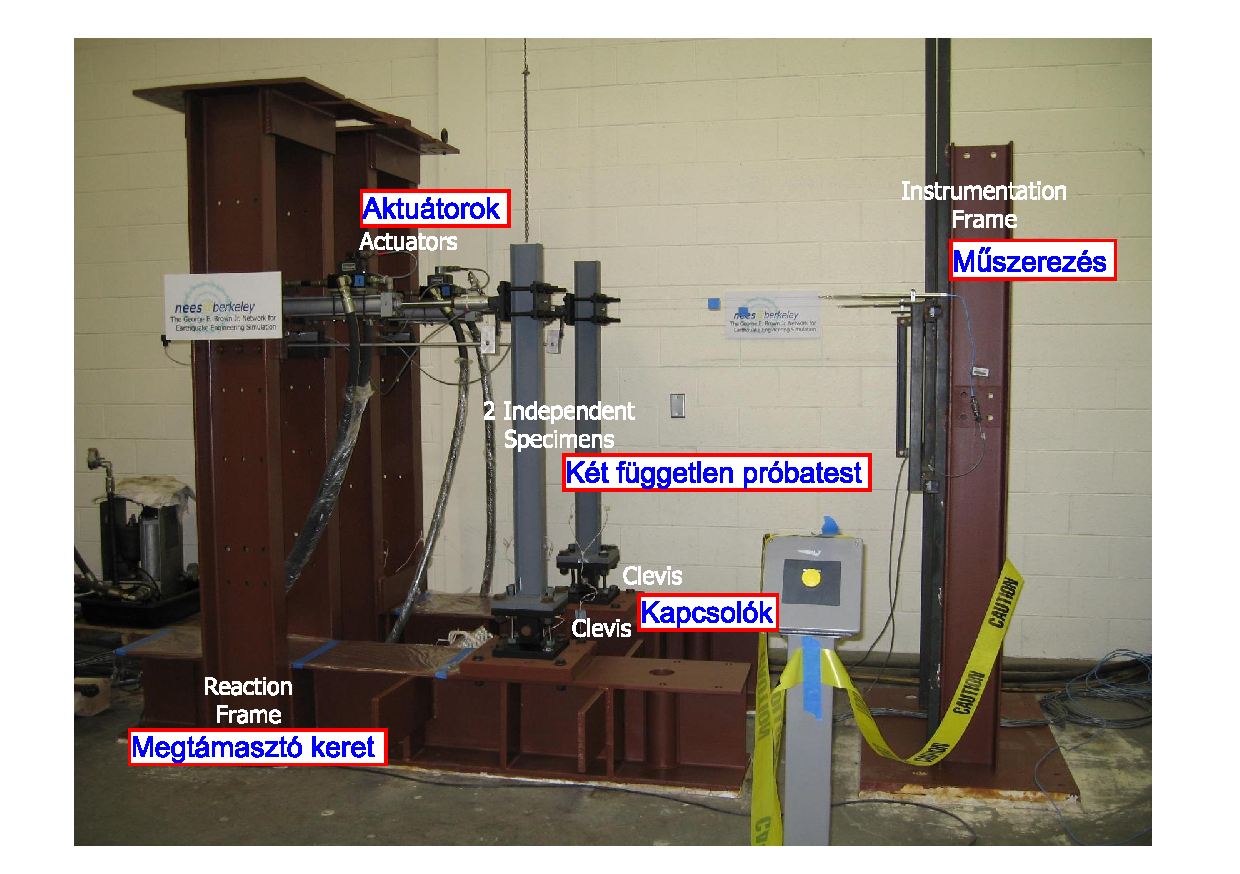
\includegraphics[width=\textwidth]{hibrid_alkalmazas.pdf}
\caption{Hibrid szimulációs kísérlet \cite{hibrid}.}
\label{fig:hibridkep}
\end{figure}


\begin{figure}[p]%
\centering
\subfigure{%
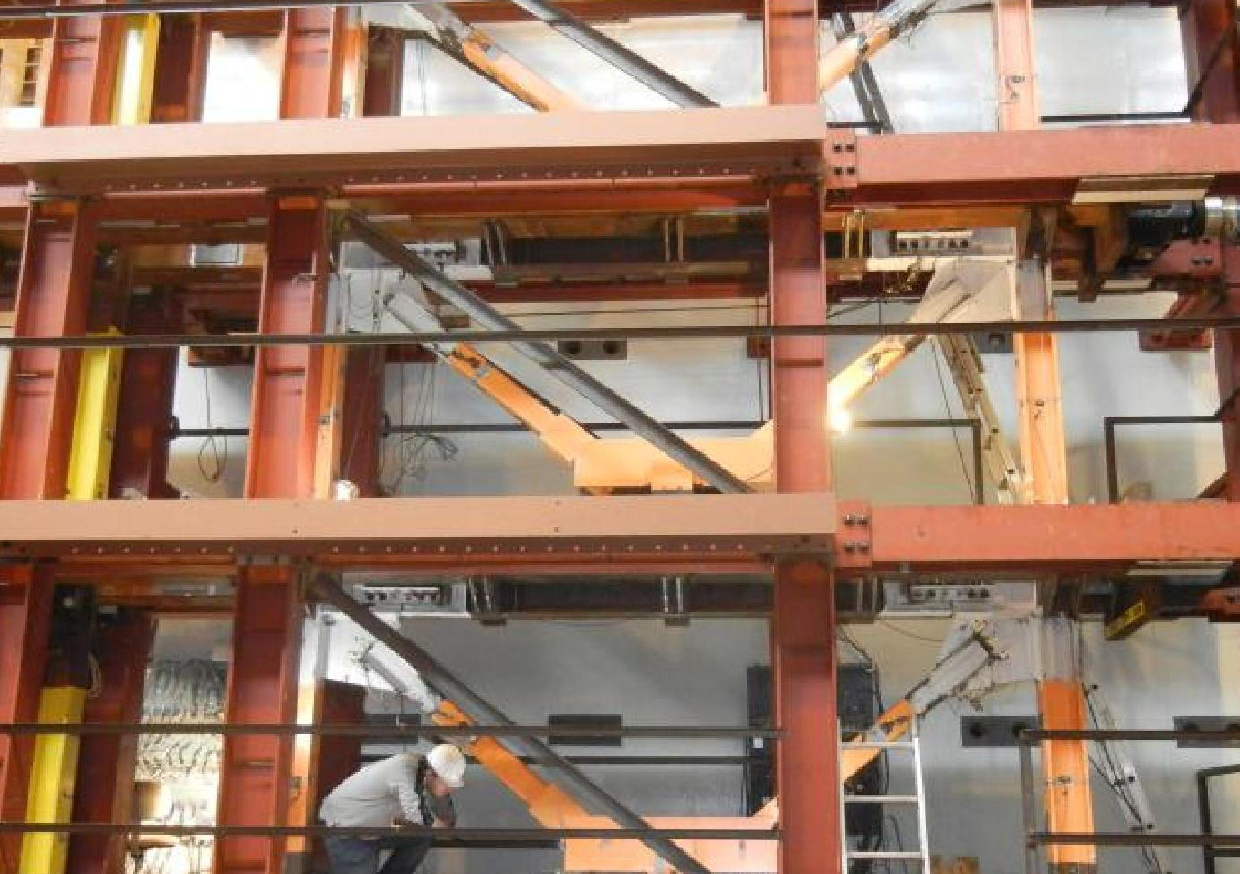
\includegraphics[width=\textwidth]{lehigh_2.pdf}}%
\\
\subfigure{%
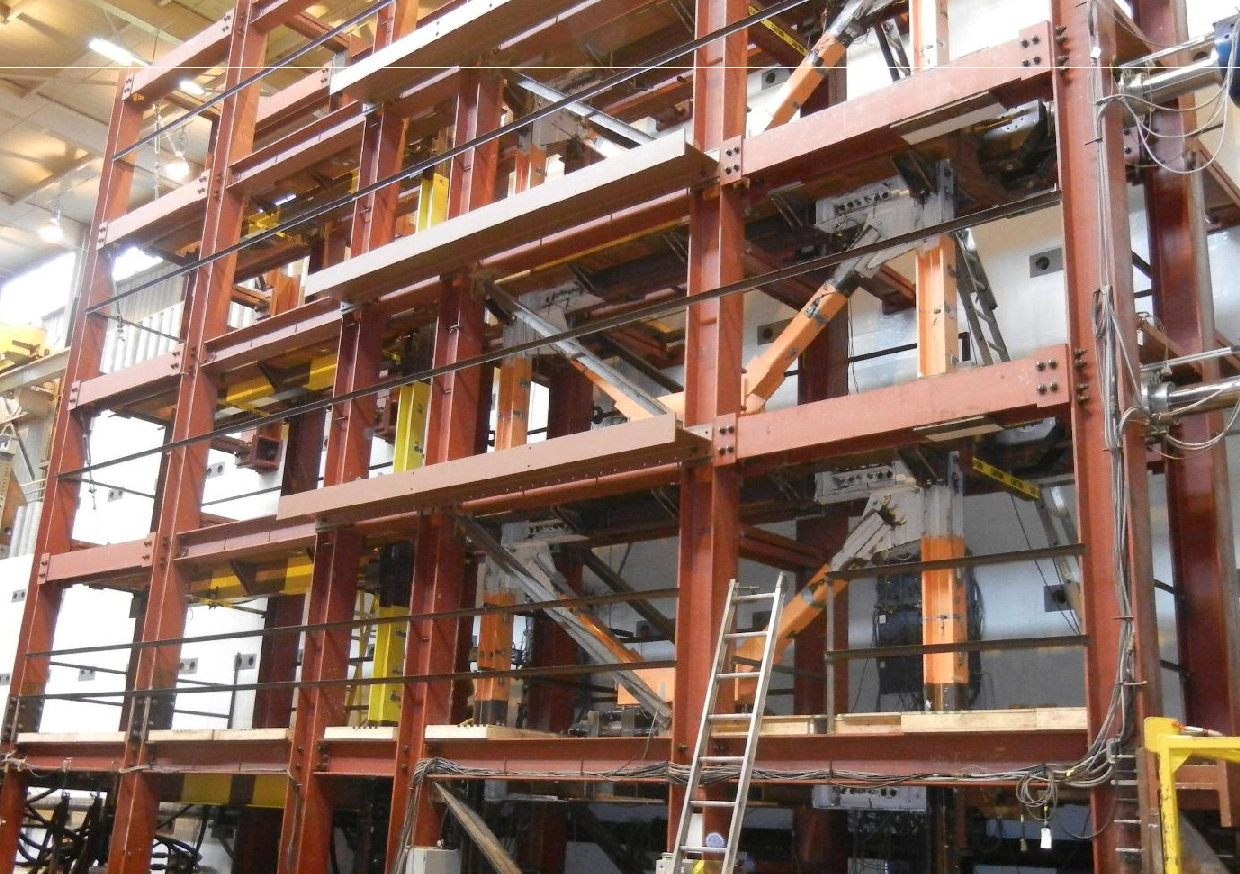
\includegraphics[width=\textwidth]{lehigh_1.pdf}}%
\caption[A Lehigh Egyetemenen végzett hibrid szimulációs kísérlet.]{A Lehigh Egyetemenen végzett hibrid szimulációs kísérlet elrendezése \cite{lehigh}.}
\label{fig:lehigh_szerk}%
\end{figure}


\newpage
\section{Előnyök és kihívások}
{\ }

A következőkben  a hibrid szimuláció főbb előnyeit mutatom be a kvázi-statikus és a rázópados vizsgálattal szemben. Emellett összefoglalom  azt a számos kihívást is, amellyel a jövőben foglalkozni kell a hibrid szimuláció kapcsán.


\subsection{Előnyök}

{\ }

A hibrid szimulációs eljárás számos előnnyel rendelkezik, mivel  a szerkezeti rendszer vizsgálatának ötvözi az analitikus és  kísérleti megközelítését, és a végrehajtható időlépték  maximum két nagyságrenddel lassabb a tényleges időléptéknél. A következő lista összefoglalja a legfontosabb előnyöket:
\begin{itemize} 
\item Egy hibrid szimulációban a teher (vagyis a mozgásegyenlet jobb oldala) analitikusan van definiálva, ami a legkülönbözőbb terhelési feltételek mellett gerjesztett szerkezetek viselkedésének vizsgálatát teszi lehetővé. A szeizmikus események, a hullámok okozta hidrodinamikus terhek, mozgó járművek miatti közlekedési terhek, szél általi aerodinamikai és a robbanásterhek mind szimulálhatók az analitikus részbe való beépítéssel, a kísérlet fizikai részeinek megváltoztatása nélkül.
\item Hibrid szimulációban lehetőség van arra, hogy egy nagyobb szerkezet részegységekre, vagyis alszerkezetekre legyen bontva: (1) a numerikus alszerkezethez a jól megértett viselkedésű szerkezeti elemek tartoznak, amelyekre biztonságosan felállítható a végeselemes modell , (2) a fizikai alszerkezethez pedig az erősen nemlineáris viselkedésű vagy numerikusan nehezen szimulálható szerkezeti elemek tartoznak, ezért ezek laboratóriumban vannak vizsgálva. A numerikus modell valós fizikai komponenssel való helyettesítése csökkenti a modellezés bizonytalanságait. A hibrid szimuláció ezért tekinthető a szerkezeti összetevők vizsgálatának egy speciális formájának is, amelynél nem kell kielégíteni olyan szigorú peremfeltételeket, mint a rázópados vizsgálatnál.
\item A teljes méretű próbatestek dinamikus vizsgálatára is lehetőség nyílik, amennyiben a hibrid szimuláció átlagos kvázi-statikus elmozdulásalapú vizsgálatként valósul meg, kiterjesztett időléptékkel végrehajtva. Továbbá a nagyméretű vizsgálatoknál megszűnnek a méretezés során felmerült nehézségek, amik a rázópadvizsgálatnál fennálltak.
\item A fizikai részegységek mérete és súlya csak a rendelkezésre álló laboratóriumi terület a padló és a megtámasztás  teherbírásától függ. Továbbá a próbatest teherbírását csak az átviteli rendszer (aktuátor) kapacitása korlátozza.
\item Mivel a hibrid szimuláció nagyobb időléptéken is végrehajtható, a kvázi-statikus vizsgáló berendezések, mint az aktuátorok, a szervoszelepek, és a hidraulikus tápegység, általában elegendőek a vizsgálathoz. Gyakran az ilyen berendezések rendelkezésre is állnak a vizsgálati létesítményekben. Ezért és amiatt, hogy fizikailag  csak a szerkezeti rendszer kritikus elemei vannak vizsgálva, a hibrid szimuláció nagyon gazdaságos laboratóriumi vizsgálati eljárás.  
\item A lassú tesztek lehetővé teszik a próbatestek pontos vizsgálatát a szimuláció közben. Lehetővé teszi a próbatest viselkedésének gondosabb megfigyelését, a károsodások megindulásának észlelését és a folyamat nyomon követését a szimuláció alatt.
\item Hibrid szimulációt a valós időléptéknél kétszer lassabb, és sokszor gyorsabb intervallum között bárhol végezhetünk a hasonlósági követelményeknek megfelelően.
\item A numerikus és a kísérleti alszerkezetek földrajzilag eloszthatók, így a szimuláció akár több különböző laborban is futhat, kihasználva a helyszínek adottságait. 
\item Az olyan hatásokat, mint a geometriai nemlinearitások, a háromdimenziós hatások, a talaj-szerkezet kölcsönhatások valamint a talajmegtámasztás hatása, mind a modell analitikus részébe kell foglalni.
\item Hibrid szimuláció alkalmazható intelligens rázópad vizsgálathoz, amelyben a szimulátor padozat valós időben irányított, olyan problémák vizsgálatára, mint a hangolt csillapító tömeg vagy a talaj-szerkezet kölcsönhatás.
\end{itemize} 

\subsection{Kihívások}

{\ }

Számos előnye és lehetősége mellett a hibrid szimulációnak szembesülnie kell számos kihívással is, ezért további kutatásokat kell folytatni a vizsgálattal kapcsolatban, és  speciális szimulációkat kell elvégezni az eredmények értékelésére és verifikálására. Néhány ilyen kihívást foglal össze a következő lista:
\begin{itemize}
\item A hibrid szimuláció fejlesztését és telepítését akadályozza a közös keretrendszer hiánya a  különböző laboratóriumokban és számítástechnikai környezetben végrehajtott vizsgálatokhoz. A vizsgálatok problémaspecifikusak, és erősen függnek a vizsgálat helyszínétől és a használt irányító- és adatgyűjtő rendszertől. Az ilyen rendkívül egyedi szoftver megvalósításokat nehéz különböző szerkezeti problémákra alkalmazni, és még nehezebb különböző laboratóriumokba átvinni. Ezért nagy szükség van egy olyan környezetfüggetlen szoftver-keretrendszerre, amely nagy teljesítményű, átlátható és könnyen bővíthető.
\item Annak biztosítására, hogy a kapott eredmények érvényesek, megbízhatóak és pontosak legyenek, rendkívül fontos, hogy a megoldás hibák miatti pontatlanságai minimalizálva, illetve javítva legyenek. A következő hibák fordulhatnak elő különböző szinteken a szimuláció során, melyek befolyásolhatják a megoldási folyamatot: (1) a diszkretizálás folyamata és az energia-disszipációról való feltételezések  miatti modellezési hibák; (2) az integráló és egyensúlyi megoldó algoritmusok okozta numerikus hibák; (3) a irányító- és átviteli rendszerek által generált kísérleti hibák; végül (4) a műszerezés és az adatgyűjtő rendszer által okozott kísérleti hibák. A kísérleti hibák energiatöbbletet vezethetnek a hibrid rendszerbe, ezáltal instabillá teszik azt,  ezért nagyon fontos minimalizálni vagy kompenzálni ezeket.
\item Az olyan hibrid szimulációk végrehajtása, ahol komplex analitikai alkotóelemek, mint az anyagi és geometriai nemlinearitások,  komplex,  rugalmatlan kísérleti alkotóelemekkel vannak kombinálva, meglehetősen bonyolult feladat. Ennek oka, hogy ezek a modellek általában implicit, iteratív integráló formulák használatát követelik, amikben a megoldási folyamat során folyamatosan ellenőrizni  kell, hogy a megoldás konvergál-e. Ráadásul a számítógépes terhelések a nemlinearitások miatt jelentősen eltérhetnek két időlépés között, megnehezítve, vagy lehetetlenné téve  a  gyors és valós idejű szimulációk végrehajtását.
\item A nagyon merev vagy felkeményedő fizikai alépítményt tartalmazó hibrid szimulációkat nehéz teljesíteni elmozdulásirányítás alatt. Ezért szükséges kihasználni az erőirányítást, a kevert erő- és elmozdulásirányítást vagy a szimuláció alatti kapcsolást az erő- és elmozdulásirányítás között. Eddig nagyon kevés kutatást végeztek ezen a területen.
\item Szükség van olyan  megközelítések kidolgozására, amik következetesen alkalmazzák a hasonlósági törvényeket akkor is, ha a szerkezeti rendszer  analitikus és kísérleti része különböző léptékű.
\item Földrajzilag elosztott hibrid szimulációk megkívánják a hálózati késésekkel és meghibásodásokkal foglalkozó, valamint a kommunikáció sebességét javító eszközöket. Ezek a funkciók elengedhetetlenek a gyenge valós idejű, földrajzilag elosztott hibrid szimulációk elvégzéséhez, ahol a valós idejű követelményeket átlagos értelemben kell kielégíteni, de nem szükséges minden egyes időlépésben. 
\item Egy másik kihívás olyan módszerek fejlesztése, amik a hibrid szimuláció pontosságát  és hatékonyságát értékelik. Ezen módszereknek lehetővé kell tenniük, hogy a hibrid szimuláció ne csak a befejezése után, hanem már a szimuláció közben is értékelhető legyen. 
\item Ahogy a hibrid modellek egyre nagyobbá válnak (egyre nő a csomópontok, elemek és szabadsági fokok száma), egyre bonyolultabbak lesznek (egyre több az anyagi és geometriai nemlinearitás), és a közel vagy ténylegesen valós idejű  vizsgálatok elterjednek, a nagy teljesítményű számítástechnikai  (High-Performance Computing - HPC)  környezet egyre nélkülözhetetlenebbé válik a hibrid szimulációk végrehajtásához. Nagy teljesítményű számítástechnikai környezetben hasznosítani lehet a többprocesszoros és/vagy többmagos párhuzamos számítástechnikai képességeket a munkaterhelés elosztására és ezáltal a teljesítmény javítására. 
\item A gyors és valós idejű hibrid szimulációkban a tehetetlenségi erőket, amik a kísérleti alkotóelemek  fizikai tömegeiből származnak, nem szabad elhanyagolni. Tehát fontos az olyan módszerek fejlesztése, amik megfelelően veszik figyelembe  ezeknek az erőknek a hozzájárulását.
\item Azért, hogy a hibrid szimuláció elérhetősége a kutatói közösség számára javuljon, hathatós, de mégis közérthető felhasználói felületet kell kidolgozni.
\end{itemize}

\section{Az eljárás  összetevői}

{\ }

A hibrid szimuláció végrehajtásához számos kulcsfontosságú összetevőre van szükség, beleértve a szoftver és hardver komponenseket is. Ezek a szimuláció során mind interakcióba lépnek. A hibrid szimuláció kulcselemeit ábrázolja a \ref{fig:hibridszim}-es ábra, és a következőkben rövid bemutatásuk olvasható.

\begin{figure}[h!]
\centering
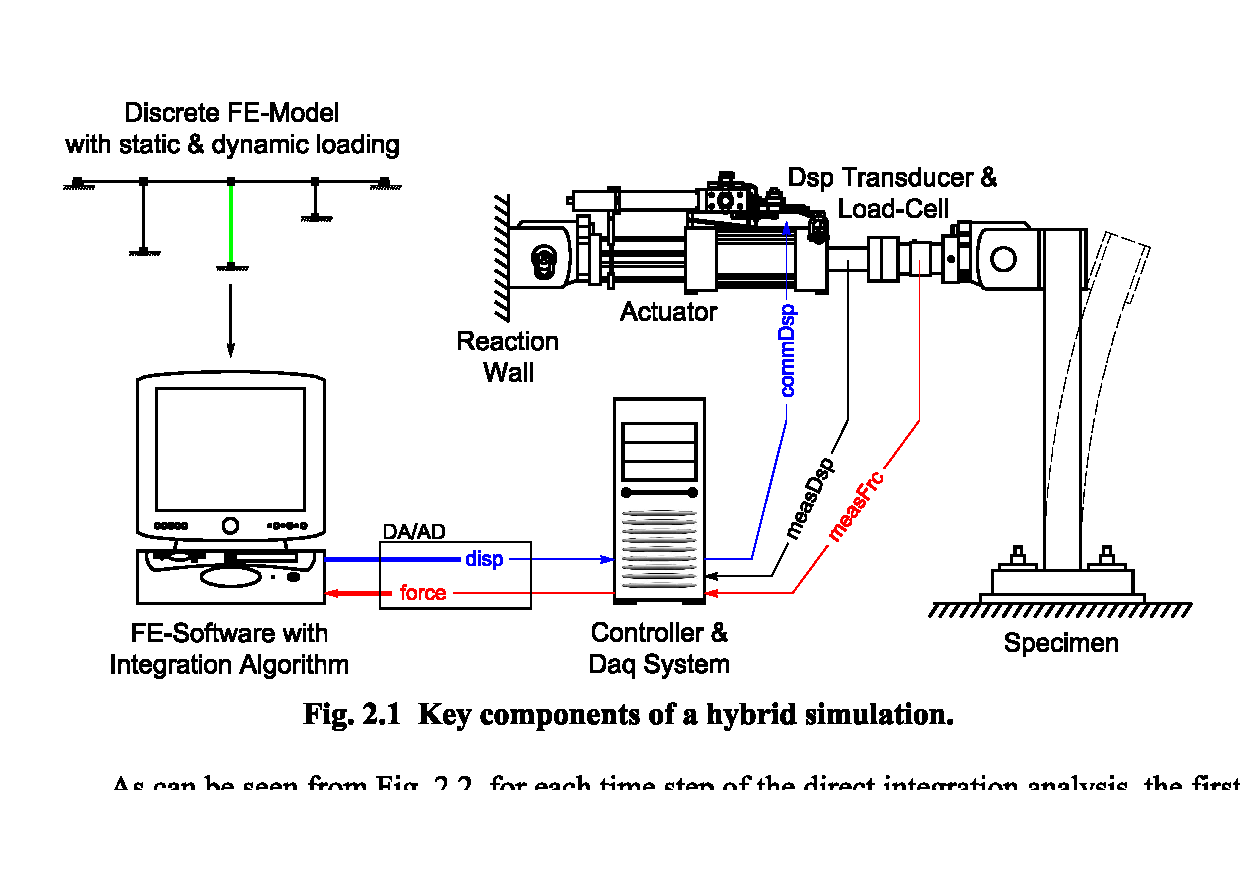
\includegraphics[trim = 0mm 30mm 0mm 0mm, clip, width=\textwidth]{hibridszim.pdf}
\caption[A hibrid szimuláció kulcselemei \cite{hibrid}]{A hibrid szimuláció kulcselemei \cite{hibrid}.(Az egyes elemek jelentésének fordítását és magyarázatát a főszöveg tartalmazza.)}
\label{fig:hibridszim}
\end{figure}

\begin{enumerate}
\item Az első komponens  a szerkezet számítógépen analizálandó diszkrét végeselemes modellje, ami tartalmazza a statikus és dinamikus terhelést is (az \ref{fig:hibridszim} ábrán: Discrete FE-Model with static and dynamic loading).  A szerkezeti analízis itt bemutatott megközelítése szerint végeselemes módszer használatos a térbeli, és  időlépéses módszer az időbeni diszkretizálásra (az \ref{fig:hibridszim} ábrán: FE-Software with Integration Algorithm). Az alternatív irányított rendszerrel való megközelítéssel összehasonlítva a végeselemes megközelítés a szerkezetépítő mérnök számára sokkal intuitívabb és könnyen kiterjeszthető megosztott hibrid szimulációk elvégzésére. A dinamikus mozgásegyenletek véges számú diszkrét szabadságfokra felírása  egy másodrendű közönséges differenciálegyenlet-rendszert eredményez, melynek szabad változója az idő.
\begin{equation}
\mathbf{M}\mathbf{\ddot{U}}_{i+1}+\mathbf{C}\mathbf{\dot{U}}_{i+1}+\mathbf{f}_s(\mathbf{U}_{i+1}) = \mathbf{P}_{i+1}-\mathbf{P}_{0,i+1}
\label{hibrid alapegyenlet}
\end{equation}
Az \eqref{hibrid alapegyenlet} egyenlet az időben diszkretizált differenciálegyenlet-rendszer a $t = t_{i+1}$ időpontra felírva, ahol az $\mathbf{M}$ a csomóponti és elemi tömegmátrixokból összeállított tömegmátrix, $\mathbf{\ddot{U}}_{i+1}$ a gyorsulásvektor a $t_{i+1}$ időpontban, $\mathbf{C}$ a képlékeny csillapítási mátrix, $\mathbf{\dot{U}}_{i+1}$ a sebességvektor a $t_{i+1}$ időpontban, $\mathbf{f}_s$ a rugalmas visszatérítő erő  az $\mathbf{U}_{i+1}$ a $t_{i+1}$ időpontban vett elmozdulásvektor függvényében, $\mathbf{P}_{i+1}$ a külső csomóponti terhek  és $\mathbf{P}_{0,i+1}$ az elemek terhei a $t_{i+1}$ időpontban.

A \ref{sec:idolepmsz} pontban bemutatott lineáris időlépéses integráló módszerek közül a \eqref{hibrid alapegyenlet} mozgásegyenlet megoldására a CR algoritmus a legalkalmasabb. A explicit, feltétel nélkül stabil eljárást a valós idejű hibrid szimulációkhoz fejlesztették, irányításelméleti módszerek alkalmazásával. 

\item A második szükséges komponens egy átviteli rendszer (Transfer System), amely egy irányítóból  és statikus vagy dinamikus aktuátorokból áll (az \ref{fig:hibridszim} ábrán: Controller, Actuator), így az időlépéses integráló formulákkal meghatározott (általában elmozdulás) növekményválaszokat alkalmazni lehet  a fizikai alépítményen. Lassú vizsgálatoknál felhasználhatók a kvázi-statikus vizsgálatokhoz is alkalmazott, relatíve olcsó eszközök. Ezek gyakran rendelkezésre állnak a szerkezetvizsgáló laboratóriumokban.

\item A harmadik fő komponens a laborban tesztelt  kísérleti próbatest, beleértve a támaszokat is (az \ref{fig:hibridszim} ábrán: Specimen, Reaction Wall), amivel az átviteli rendszer aktuátorai kapcsolódnak.

\item A negyedik és egyben utolsó komponens egy adatgyűjtő rendszer (az \ref{fig:hibridszim} ábrán: Daq System), amely olyan elemeket tartalmaz, mint az elmozdulás jeladók, az erőmérő cellák (az \ref{fig:hibridszim} ábrán: Dsp Transducer \& Load-Cell) és a gyorsulásmérők (Accelerometers). Az adatgyűjtő rendszer felelős a próbadarab válaszának méréséért és kísérleti adatként való továbbításáért a numerikus alépítmény felé, hogy a következő időlépéshez tartozó megoldás számítható legyen.
\end{enumerate}

 A hibrid szimulációs eljárásokra fejlesztették az OpenFresco (Open-source Framework for Experimental Setup and Control) környezetfüggetlen szoftver keretrendszert. Az OpenFresco  a hibrid szimulációs eljárásokban a végeselemes modellt köti össze az irányító és adatgyűjtő rendszerrel, így megkönnyíti a laboratóriumi kísérletek  elvégzését. A végeselemes modell készítésére ebben a környezetben a legelterjedtebb az OpenSEES szoftver. A programot kifejezetten szerkezetek viselkedésének vizsgálatára fejlesztették földrengés hatására  alatt.

%Mivel a szimuláció kulcselemei végeselemes megközelítés alkalmazásával lettek bemutatva,  adott a direkt integrálás végrehajtásának szempontjából  szükséges  vizsgálati eljárás. Az eljárás részleteinek egyszerűsítése végett a nemlineáris helyett lineáris egyensúlyi megoldó algoritmus kerül alkalmazásra. A vizsgálati eljárás folyamatábráját mutatja a \ref{hibrid folyamat}-es ábra. 

%Amint a \ref{hibrid folyamat}-es ábrából látható, a direkt integrálás minden egyes időlépésében az első művelet az új próba válaszmennyiségek (elmozdulások, sebességek és gyorsulások) meghatározása. Ezután a terhelés és a vizsgálati idő növekszik, és az új próba válaszmennyiségek lesznek elküldve  az analitikus és a kísérleti alszerkezetnek. Az analitikus alszerkezet tárolja az új válaszmennyiségeket, így ezek később meghatározhatják a kiegyensúlyozatlan terheket. Másrészt  a kísérleti alszerkezet kommunikál az átviteli rendszerrel a laborban, ami elkezdi az új elmozdulásokat végrehajtani.

\section{A helyi és a földrajzilag megosztott eljárás összehasonlítása}

{\ }

Ha a hibrid szimuláció előnyeit felsorakoztatjuk, láthatjuk, hogy  egy nagyon sokoldalú vizsgálati módszer, és ez sok különböző alkalmazási módot tesz lehetővé. Ezért érdemes kategorizálni a fő alkalmazási módokat és meghatározni a hozzájuk  kapcsolódó fogalmakat.

A kategorizálás első módja a szerkezeti alegységek és a különböző elemek  csoportosítása földrajzi megosztottságuk szerint. A helyi vagy lokális hibrid szimulációban a numerikus analízis és a kísérleti vizsgálat elvégzése ugyanazon a helyen, vagyis ugyanabban a laboratóriumban történik.  Mivel a végeselemes analízis  hardvere, az irányító rendszer, az adatgyűjtő rendszer mind ugyanott helyezkedik el, a csatlakozásuk megoldható helyi nagysebességű hálózati körön keresztül. Ezek drasztikusan csökkentik a késedelmeket, és lehetővé teszik a folyamatos vagy akár a valós idejű hibrid szimulációk végrehajtását. Így a helyi hibrid szimulációnak többnyire nem akadálya a szerkezeti egységek közötti kapcsolat hiánya, viszont az összes szükséges alkatrész egy laboratóriumban való elhelyezése komoly nehézségekbe ütközhet.

Ezzel szemben a földrajzilag megosztott hibrid szimulációban a szerkezet különböző részei különböző helyszíneken vannak vizsgálva és  elemezve. Ez azt jelenti, hogy a modell analitikus részei egyszerre több számítógépen is elemezhetők, és  a hibrid modell fizikai részei egyszerre több laboratóriumban is vizsgálhatók. Mivel néhány vagy az összes alegység szétszórtan helyezkedik el,  összekapcsolásukra csak nagy kiterjedésű hálózatok használhatók. Ezek általában nagyobb késéseket okoznak, mint a helyi nagysebességű hálózatok, így a gyors hibrid szimulációk végrehajtása  nagy kihívást jelent. Ráadásul szükség van egy eszközre, ami a túlzottan nagy hálózati késésekkel és a meghibásodásokkal foglalkozik. Azonban a modell  kijelölt alegységekre bontásával valamint laboratóriumok és számítási helyek hálózatán belüli eloszlásával  lehetőség nyílik a különböző adottságú helyszínek optimális kihasználására. 

\section{A lassú, a gyors és a valós idejű vizsgálatok összehasonlítása}

{\ }

A hibrid szimuláció másik fontos jellemzője  a vizsgálat végrehajtásának sebessége. A lassú vizsgálatokat a valós időléptéknél  akár két nagyságrenddel nagyobb időléptékkel hajtják vére,  míg a valós idejű vizsgálatokat a tényleges időléptékkel azonos vagy annál kisebb időléptékkel kell elvégezni a hasonlósági követelményektől függően. Így a hibrid szimuláció különböző aspektusait a végrehajtás sebességének függvényében alaposabban kell figyelembe venni és kezelni. A lassú vizsgálatnál nagyon fontos, hogy a fizikailag vizsgált szerkezeti részek nem mutathatnak sebességfüggő viselkedést kivéve, ha ezt az analitikus részben kompenzálják. Ezenkívül fontos az  aktuátor folytonos mozgásával járó megszakítás nélküli végrehajtás, a relaxációs erő és a rúd szétcsúszásának elkerülése érdekében. Másrészt a gyors hibrid szimulációhoz elengedhetetlen a fizikai részek által generált  tehetetlenségi és  csillapító erők megfelelő számítása vagy kompenzálása. Emellett fontos annak felismerése, hogy az ilyen vizsgálatokhoz nagy erejű dinamikus aktuátorok nagy akkumulátorral és hidraulikus szivattyú rendszer szükségesek, ezáltal az aktuátorok pontos irányítása sokkal nehezebbé válik a tehetetlenségi erő visszacsatolások miatt.

A hibrid szimuláció során megoldandó mozgásegyenletek némileg eltérő formákat vesznek fel a végrehajtás sebességétől függően. A lassú teszteknél nem keletkeznek tehetetlenségi erők a fizikai alegységekben, ezért az egész szerkezet tömeg és viszkózus csillapítási mátrixa numerikusan kezelhető, ugyanis a kísérleti visszatérítő erő  nem tartalmaz semmilyen inerciális vagy viszkózus csillapító erő hozzájárulást.  Így a tömeg és a csillapítási mátrix közvetlenül előállítható  az analitikus és kísérleti alszerkezet  csomópontjainak és szerkezeti elemeinek együttes figyelembevételével. 
 
Ezzel ellentétben, ha a hibrid szimulációt gyorsabban hajtják végre,  tehetetlenségi és viszkózus csillapító erők keletkeznek a szerkezet fizikailag vizsgált részeiben, ezeket figyelembe kell venni a kísérleti visszatérítő erő vektorában. A visszatérítő erő számításához szükséges tömeg és csillapítási mátrixokat a kísérleti alszerkezet alapján állítjuk össze, a gyorsulások és sebességek vektorait pedig a kísérleti részeken mérjük.

Ha elérjük a valós idejű sebességet, a kísérleti alszerkezetre a  számított gyorsulások és sebességek hatnak (a hasonlósági követelmények figyelembevételével). Így a mozgásegyenletben a tömeg és csillapítási mátrixokat elég csak a numerikus alszerkezetből számolni, a visszatérítő erőt pedig elég a kísérleti alszerkezet alapján előállítani, ami tartalmazza a szerkezet fizikai részeinek tehetetlenségi és csillapítási erőit. A kísérleti visszatérítő erő vektor teljes egészében előállítható a mért erők értékeiből. Viszont ha a valós idejű szimulációt intelligens rázópadkísérlethez alkalmazzák, ahol  nagyobb alegységeket vizsgálnak a kísérleti platón, a kísérleti visszatérítő erő nem a relatív válaszmennyiség függvénye, ehelyett az abszolút válaszmennyiséget kell a rázópad irányító rendszerének küldeni.  



\section{A hibrid szimuláció értékelése}

{\ }

Tanulmányomban bemutattam a hibrid szimulációs eljárást, és ismertettem előtérbe kerülésének okait. Összefoglaltam az előnyeit más kísérleti eljárásokkal szemben, valamint a szimuláció megvalósításához kapcsolódó kihívásokat. Bemutattam az eljárás kulcselemeit, és azt, hogy milyen műszerekkel valósítható meg. Jellemeztem az eljárást földrajzi megosztottság  és a szimuláció sebessége szerint. Ezek  alapján a hibrid szimulációs eljárás pontos, viszonylag könnyen megvalósítható, könnyen variálható  és költséghatékony kísérleti módszer, ami alkalmas a nagyobb építőmérnöki szerkezetek dinamikus teljesítményének vizsgálatára. 

 A következő fejezetben bemutatom a hibrid szimulációs eljárásra fejlesztett programomat. A valós idejű  szimulációk végrehajtására a CR algoritmus a legalkalmasabb, így  a programban én is ezt  alkalmaztam a numerikus számítások végrehajtására.











